\section{Testbench Architecture}

The testbench of the MCE uses a grey box view of the design.
Meaning, that the current state of the DUT is not only determined by the information gathered at the interfaces, but also by internal signals.
On the one hand this has the downside, that the testbench is dependent upon the internal structure of the design.
So internal changes in the design can require adjustments of the testbench, which typically should be avoided.
On the other hand this makes it easier to check the behavior of the DUT.
Since the interfaces of the design provide only limited information about the current state of the design itself, the grey box view is necessary to collect enough covergage data to verify the engine.\\ 
Structural the testbench of the MCE consists of two interface UVCs, a module UVC and a virtual sequence driver (figure~\ref{fig:mce_tb}).\\
The interface UVCs are used to handle the interfaces of the engine.
Thereby, the CSR UVC is responsible for the memory interface.
The other interfaces are grouped together in the \emph{ProgramFlow} UVC and a virtual sequence driver is used to coordinate the interaction between the individual interfaces.\\
The transactions produced by the interface UVCs are sent to the module UVC to check the behavior of the MCE across the different interfaces.
The module UVC additionally collects data of the internal state of the design.



\begin{figure}[htb]
 \centering
 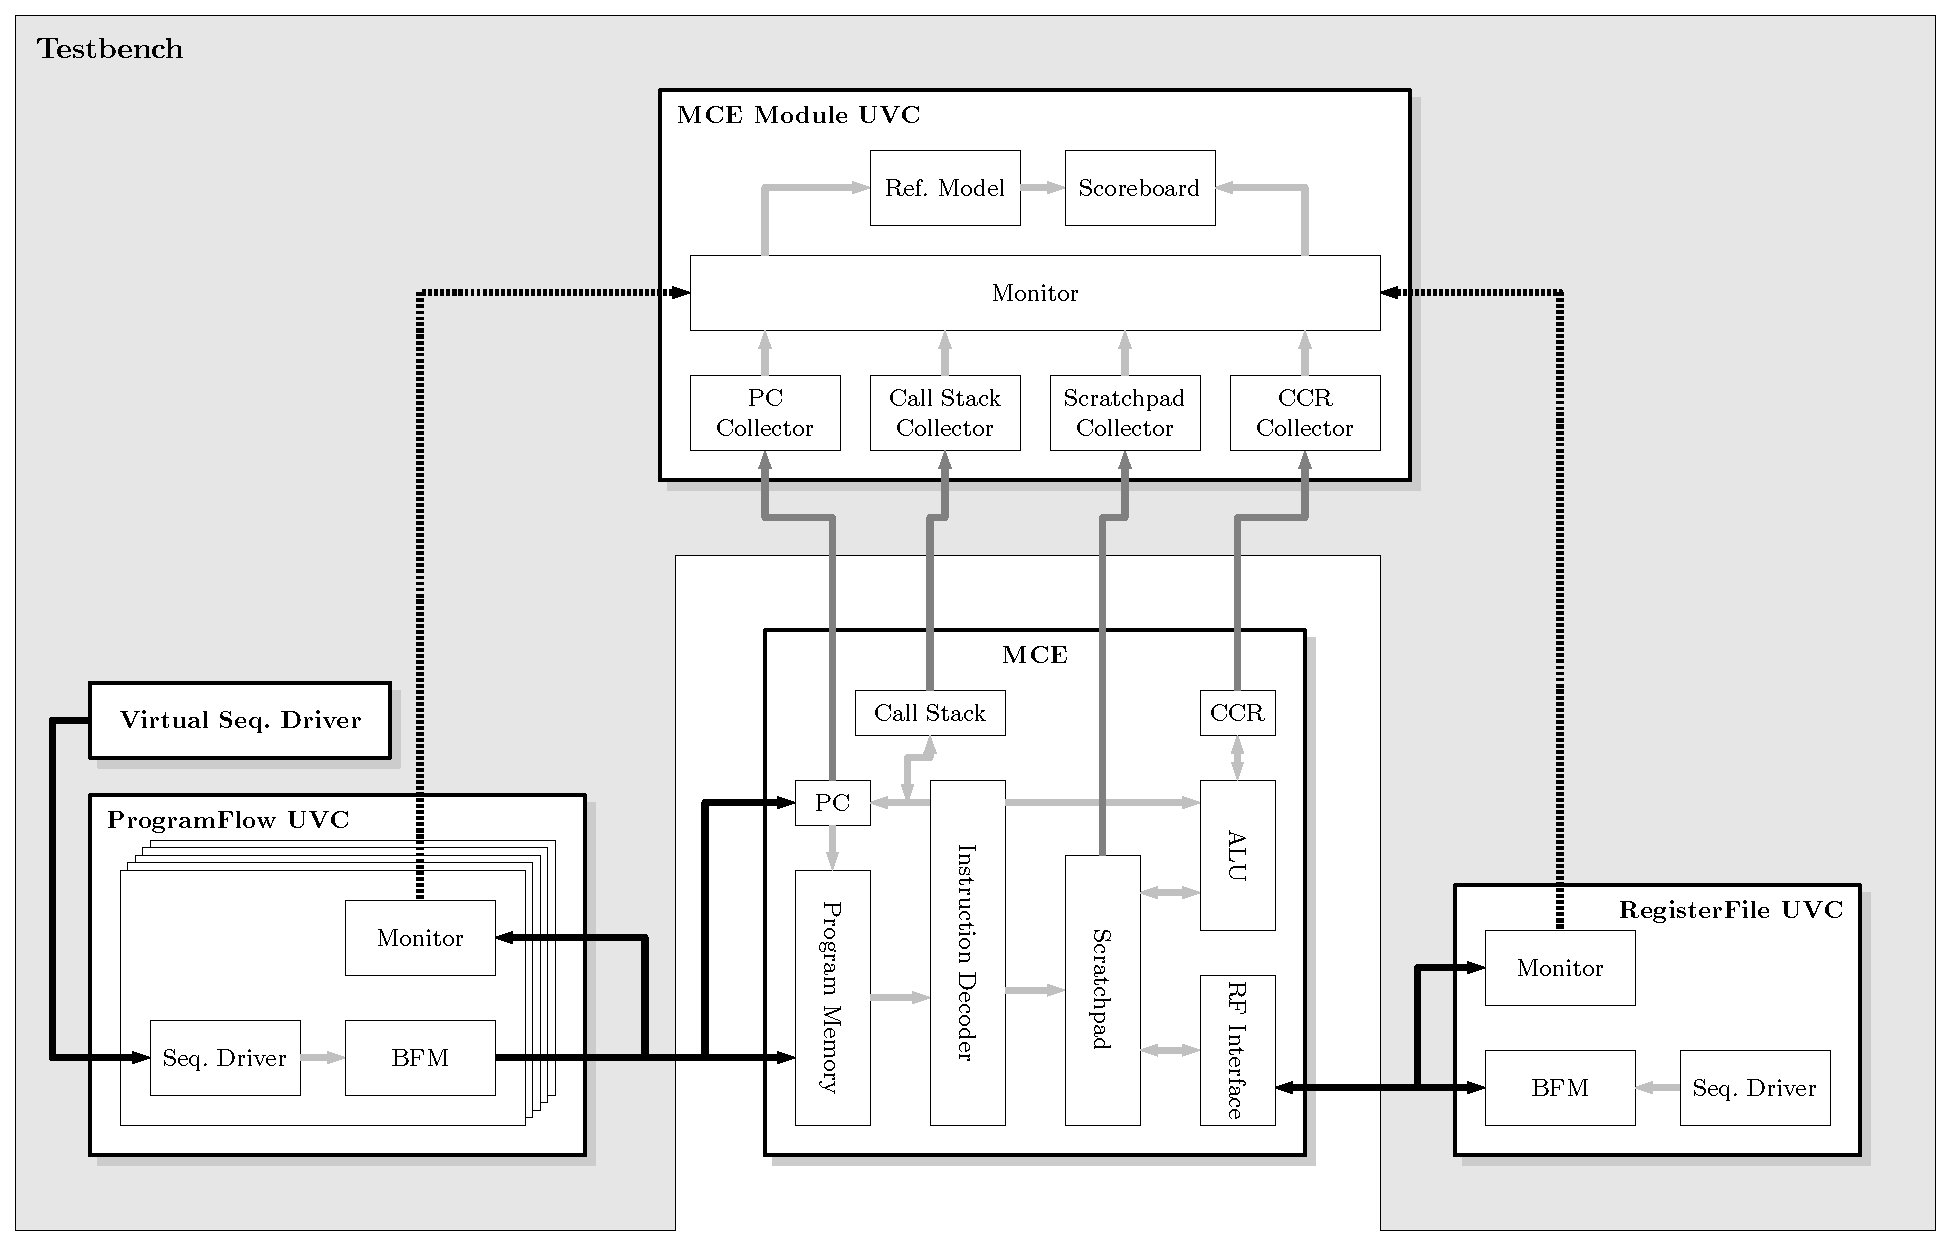
\includegraphics[width=1.0\textwidth,angle=0]{images/mce_tb}
 \caption{MCE Testbench}
\label{fig:mce_tb}
\end{figure}

\subsection{ProgramFlow Interface UVC}

The ProgramFlow interface UVC groups multiple interfaces of the MCE. 
It handles the instruction memory, external condition code bits, call stack overflow, start and done interface.
Thereby each interface has its own agent.
These agents are described in the following sections.

\subsubsection{Instruction Memory Agent}

\subsubsection{External Condition Code Bits Agent}

\subsubsection{Call Stack Overflow Agent}

\subsubsection{Start Agent}

\subsubsection{Done Agent}

\subsection{CSR Interface UVC}

The external memory interface is handled in the CSR interface UVC.
Its monitor samples the individual signals of the interface and creates an sequence item for each CSR access with the collected data.
This item is then sent to the module UVC via a TLM port.\\
When the MCE starts a transaction, the UVC has to respond to this request.
So if the monitor notices, that a transaction was started, it emits an event, causing the sequence driver to generate the response.
Since a memory access can take multiple clock cycles to complete, first a random number of up to 10 clock cycles is waited.
After that the UVC sends the access complete signal and additionally random data is returned for a read transaction.
Furthermore there is a chance, that the transaction is completed indicating an invalid address in addition to the access complete signal.

\subsection{MCE Module UVC}

The module UVC of the MCE has knowledge of the desired behavior of the DUT.
It uses a reference model to predicts the behavior of the engine for a given set of stimuli.
In the scoreboard the results are then matched against the data received from the interface UVCs and its own collectors.

\begin{figure}[htb]
 \centering
 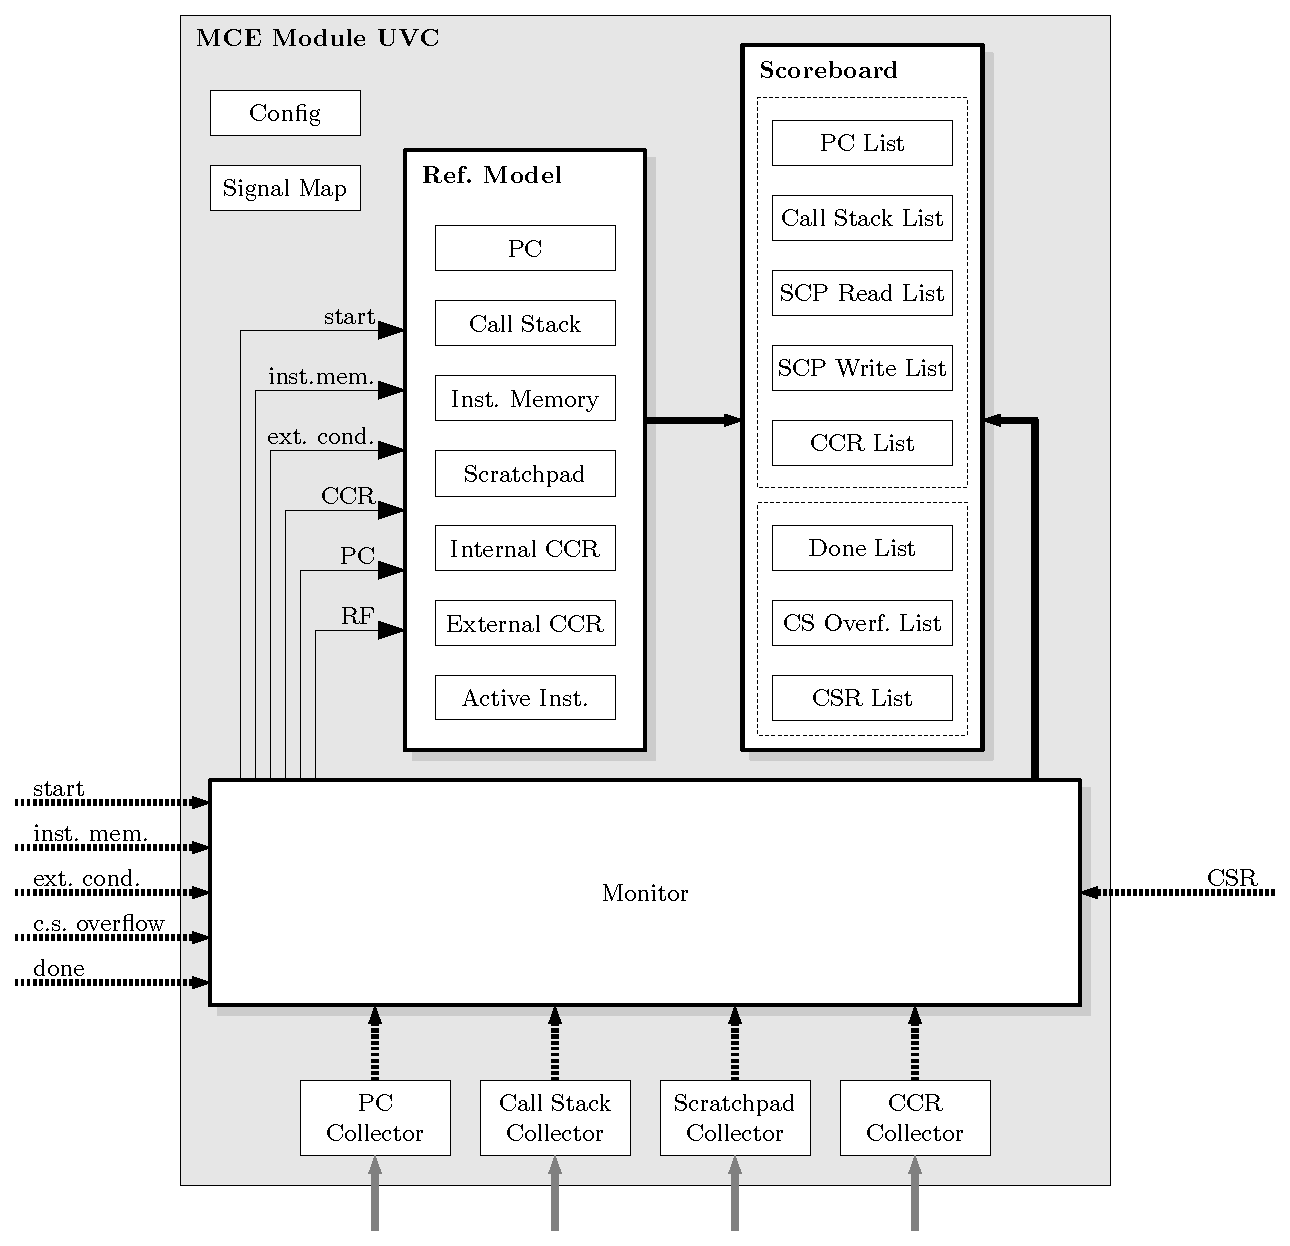
\includegraphics[width=1.0\textwidth,angle=0]{images/mce_module_uvc}
 %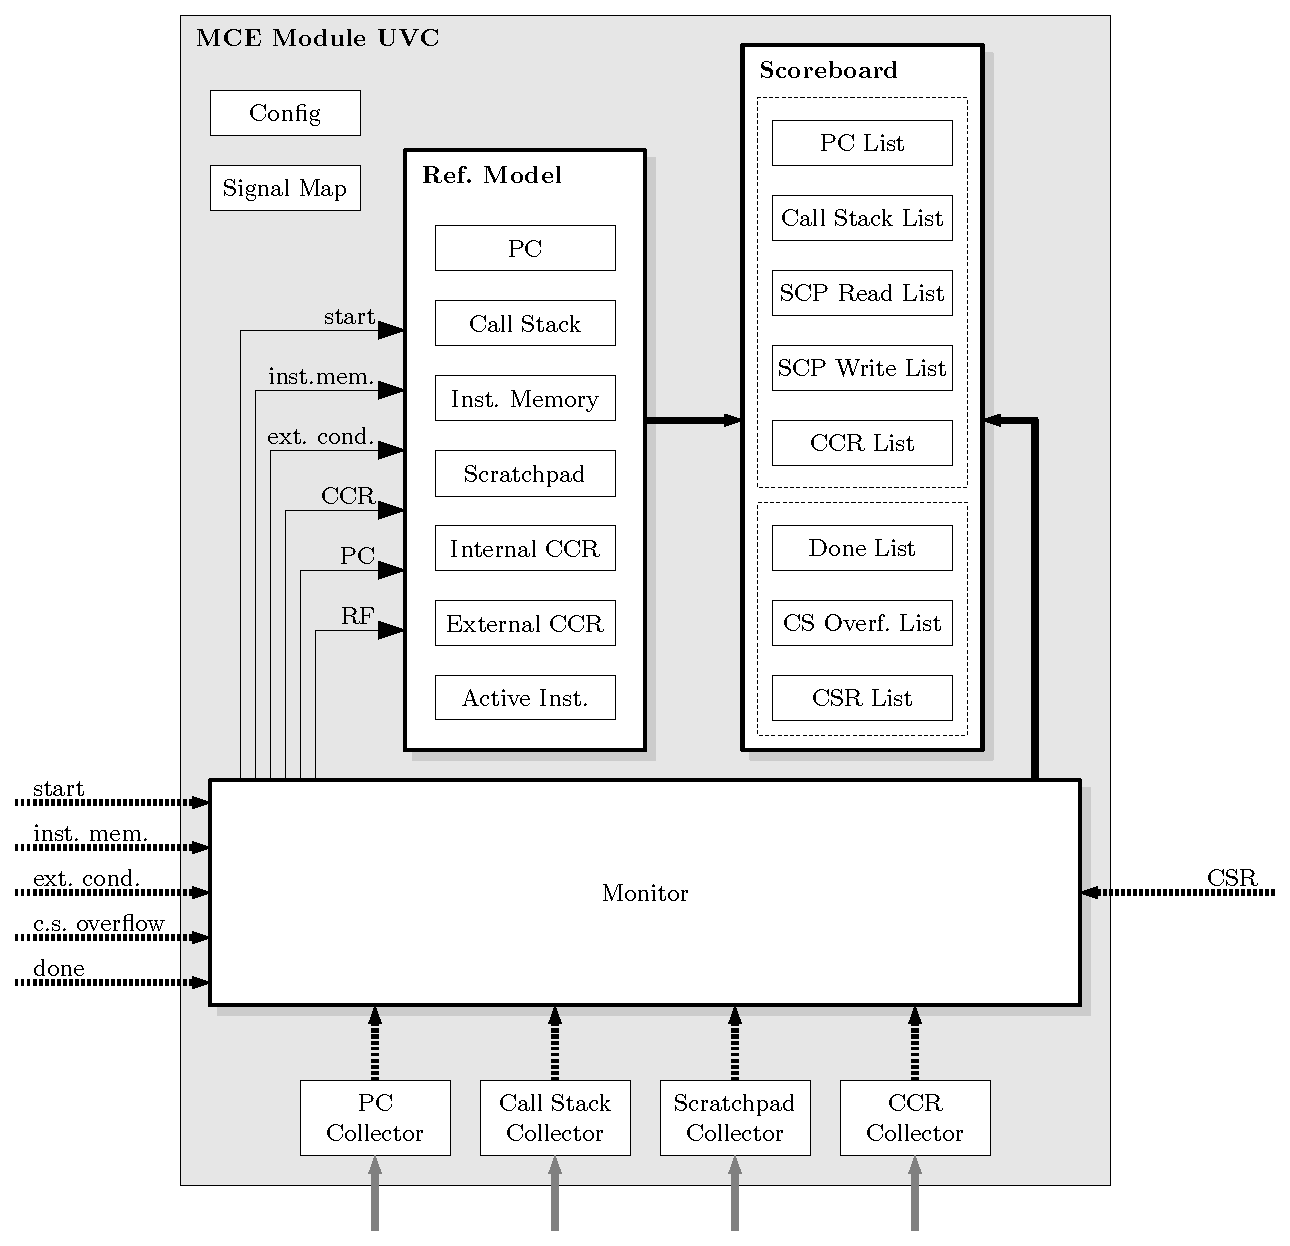
\includegraphics[scale=1.0]{images/mce_module_uvc}
 \caption{MCE Module UVC}
\label{fig:module_uvc}
\end{figure}

\subsubsection{Collectors}

\paragraph{Program Counter Collector}

\paragraph{Call Stack Collector}

\paragraph{Scratchpad Collector}

\paragraph{Condition Code Register Collector}

\subsubsection{Monitor}

\subsubsection{Scoreboard}

\subsubsection{Reference Model}

\paragraph{List of Active Instructions}

\paragraph{Instruction Execution Flow}

\paragraph{Stall Barrier}

\paragraph{Register File Read Transactions}

\paragraph{CCR Write Transactions}

\subsection{Virtual Sequence Driver}

\subsection{Test Library}